\documentclass[tikz,border=3mm]{standalone}
\usepackage[T1]{fontenc}
\usepackage[scaled=0.95]{helvet}
\renewcommand{\familydefault}{\sfdefault}
\usepackage{pgfplots}
\usepackage{xcolor}
\usetikzlibrary{arrows.meta}
\pgfplotsset{compat=1.18}
\definecolor{ink}{HTML}{14213D}
\definecolor{blue}{HTML}{0B5CAD}
\definecolor{rulegrey}{HTML}{C9CED6}
\definecolor{cfull}{HTML}{1F6FB2}
\definecolor{cnover}{HTML}{8DBBE3}
\definecolor{cbzero}{HTML}{E08A2E}
\definecolor{cbone}{HTML}{B5443A}
\definecolor{crev}{HTML}{F2C14E}
\definecolor{good}{HTML}{2E7D4F}
\definecolor{bad}{HTML}{C0392B}
\definecolor{hilite}{HTML}{FFE066}
\definecolor{codebg}{HTML}{1E2329}
\pgfplotsset{poster/.style={font=\sffamily\fontsize{14}{17}\selectfont,
  every axis label/.append style={font=\sffamily\fontsize{15}{18}\selectfont},
  every tick label/.append style={font=\sffamily\fontsize{13}{16}\selectfont},
  major tick length=2mm, axis line style={line width=0.8pt, black!60},
  tick style={black!60}, grid style={black!12,line width=0.6pt}}}
\begin{document}

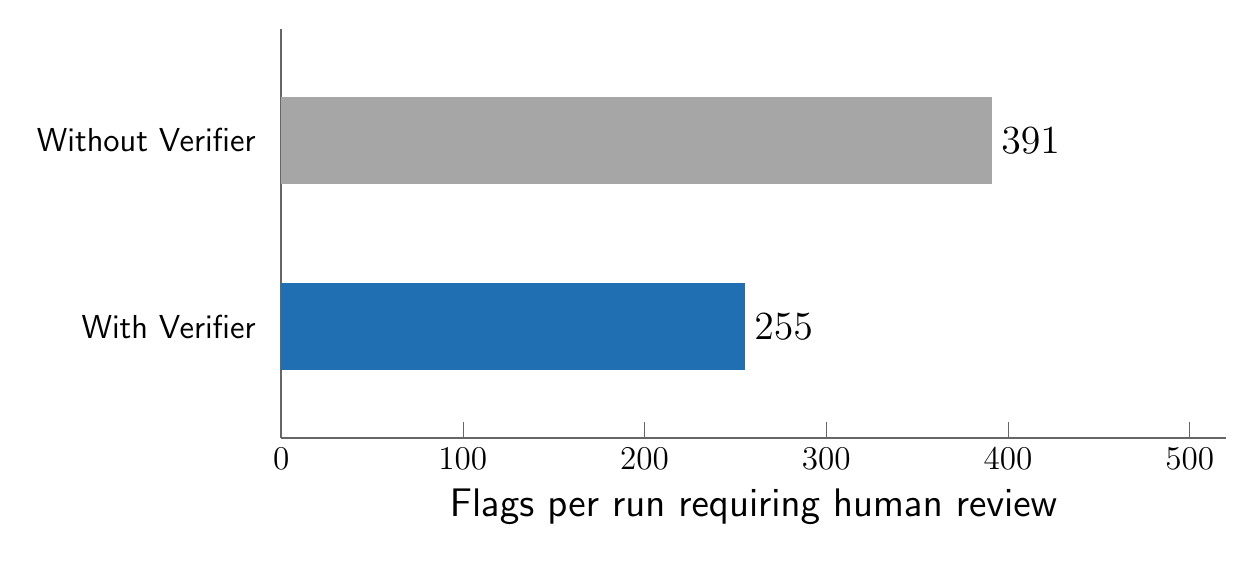
\begin{tikzpicture}
\begin{axis}[poster, width=120mm, height=52mm, scale only axis,
  xbar, bar width=11mm, bar shift=0pt, xmin=0, xmax=520, ytick={1,2}, yticklabels={With Verifier,Without Verifier},
  ymin=0.4, ymax=2.6, xtick={0,100,200,300,400,500},
  xlabel={Flags per run requiring human review}, axis x line*=bottom, axis y line*=left, ytick style={draw=none},
  nodes near coords, every node near coord/.append style={anchor=west, font=\sffamily\fontsize{15}{18}\selectfont\bfseries}]
\addplot[fill=cfull,draw=none] coordinates {(255,1)};
\addplot[fill=black!35,draw=none] coordinates {(391,2)};
\end{axis}
\end{tikzpicture}
\end{document}